\subsection{Explicación formal del problema}
\label{subsec:problema3}
Sea el conjunto de puntos del primer cuadrante $C = \{(x_1, y_1), \hdots, (x_n, y_n)\}$. Se desea hallar alguna partición, $P$, del mismo que cumpla las siguientes dos propiedades:
\begin{enumerate}
  \item $P$ tiene cardinalidad mínima;
  \item $(\forall X \in P) (\exists r$ : semirrecta$) (\forall punto \in X)$ $punto \in r$. Esto es, que cada conjunto de la partición solo puede tener puntos que pertenecen a una misma semirrecta (sea cual sea esta). 
\end{enumerate}
Notar que la segunda condición no restringe la posibilidad de que $r$ atraviese puntos de otro conjunto de la partición. 

Por ejemplo, consideremos $C=\{(3,2), (3,5), (3,7), (5,6), (7,4)\}$. Tomemos la partición $P' = \{\{(3,2), (3,5)\}, \{(3,7)\},\{(5,6), (7,4)\}\}$. Para ver si $P'$ es solución de nuestro problema grafiquemos los puntos y trazemos una posible configuración de semirrectas correspondiente a la partición, como en la figura (\ref{fig:ej3-2})\footnote{En esta sección los gráficos usarán la siguiente convención: los puntos considerados están marcados con círculos y cuadrados, representando estos últimos el origen de las semirrectas. }. Viendo esto es claro que podría atravesarse todos los puntos con solo dos semirrectas en lugar de 3. Inspirados en la figura (\ref{fig:ej3-1}) deducimos que una solución es $P = \{\{(3,2), (3,5), (3,7)\},\{(5,6), (7,4)\}\}$. En este caso puntual además resulta que es la única solución posible (teniendo en cuenta que no nos importa el orden de los puntos por ser conjuntos). Aunque esto en general no vale, como se ve por ejemplo en las figuras (\ref{fig:ej3-3}) y (\ref{fig:ej3-4}), donde las elecciones de semirrectas inducen particiones claramente distintas.

\begin{figure}[H]
\centering
\begin{minipage}{0.49\textwidth}
  \centering
    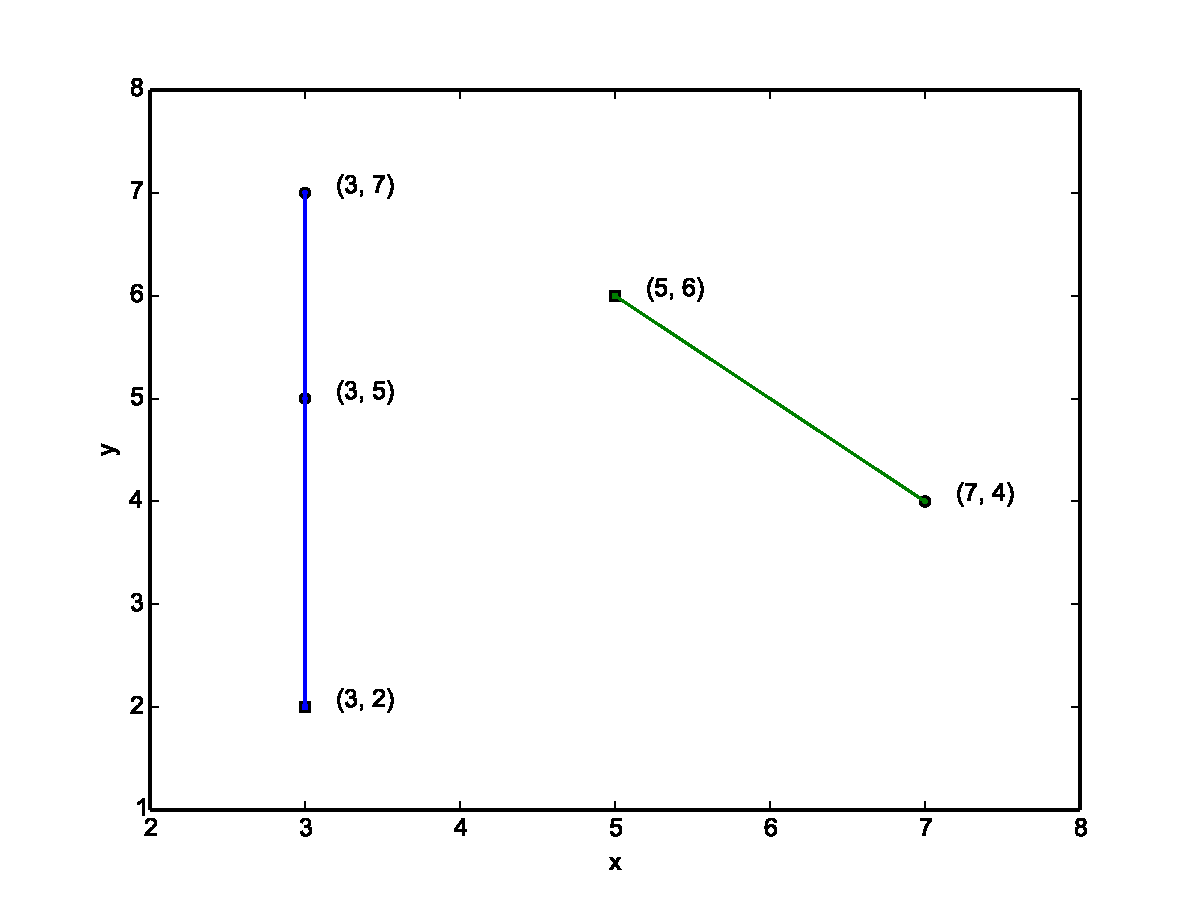
\includegraphics[width=1\textwidth]{img/ejemplos/ej3-1.pdf}
  \caption{\footnotesize Posible elección de semirrectas para la partición $P$.}
  \label{fig:ej3-1}
\end{minipage}%
\hspace{0.01\textwidth}
\begin{minipage}{0.49\textwidth}   
  \centering
    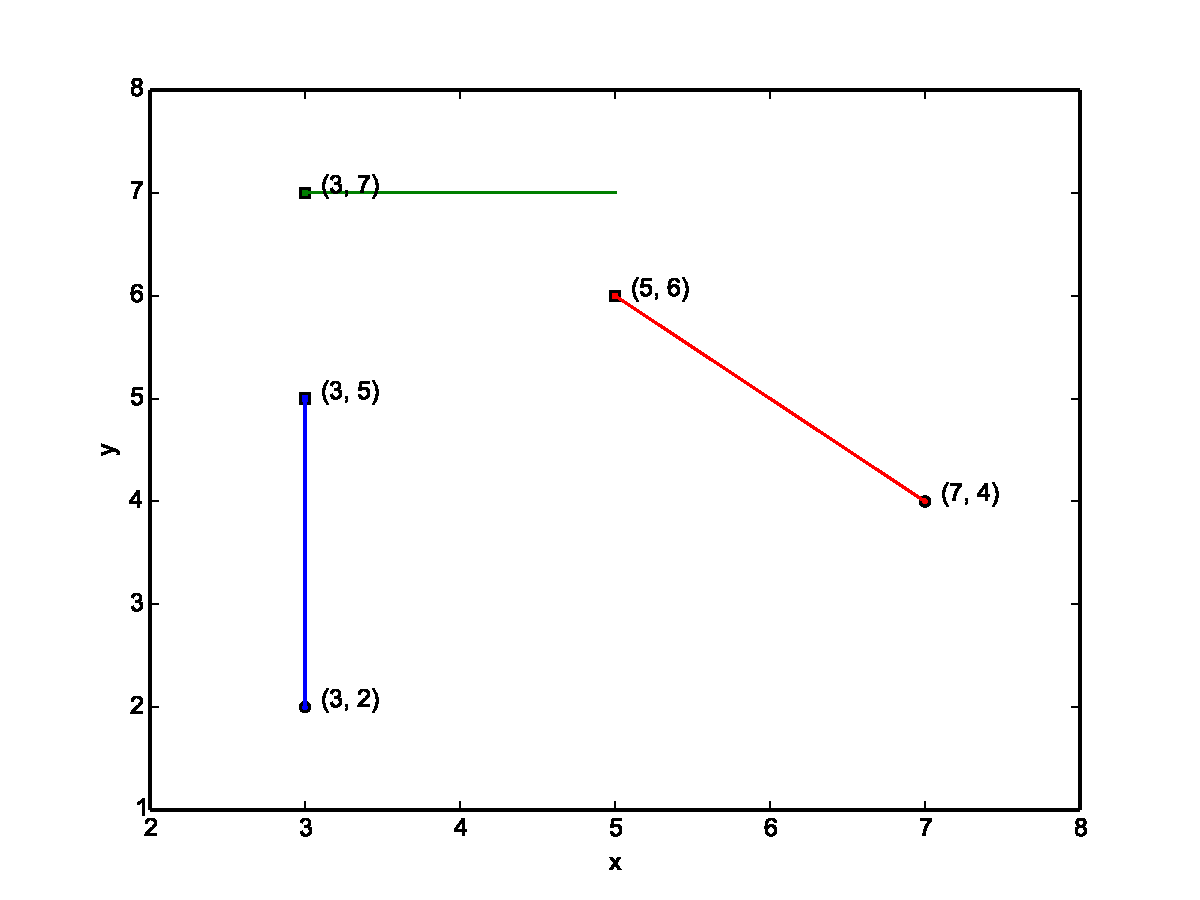
\includegraphics[width=1\textwidth]{img/ejemplos/ej3-2.pdf} 
  \caption{\footnotesize Posible elección de semirrectas para la partición $P'$.}
  \label{fig:ej3-2}
\end{minipage}%
\end{figure}

\begin{figure}[H]
  \centering
  \begin{minipage}{0.49\textwidth}
  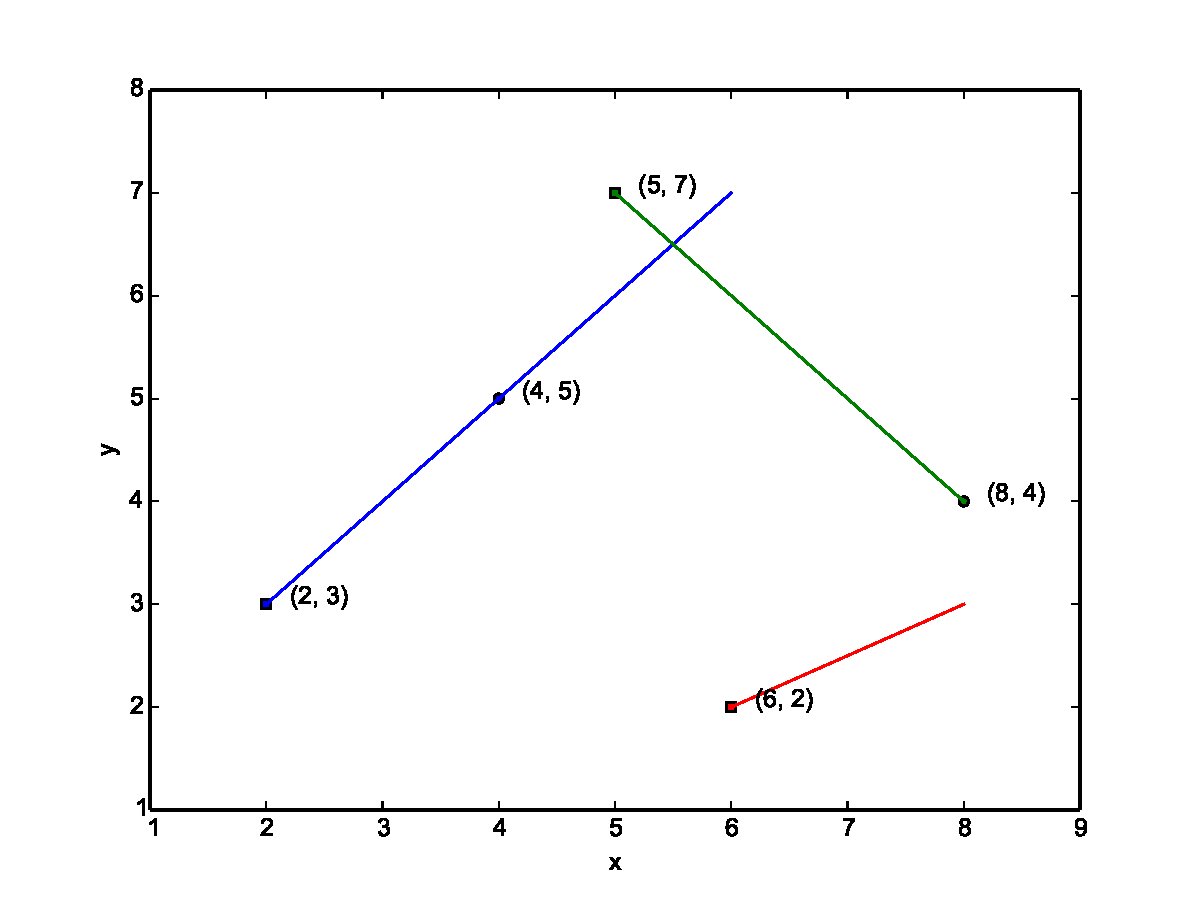
\includegraphics[width=0.85\textwidth]{img/ejemplos/ej3-3.pdf}
  \caption{\footnotesize Solución óptima para un conjunto dado de 5 puntos, donde no hay 3 puntos alineados.}
  \label{fig:ej3-3}
  \end{minipage}%
  \hspace{0.01\textwidth}
  \begin{minipage}{0.49\textwidth}
  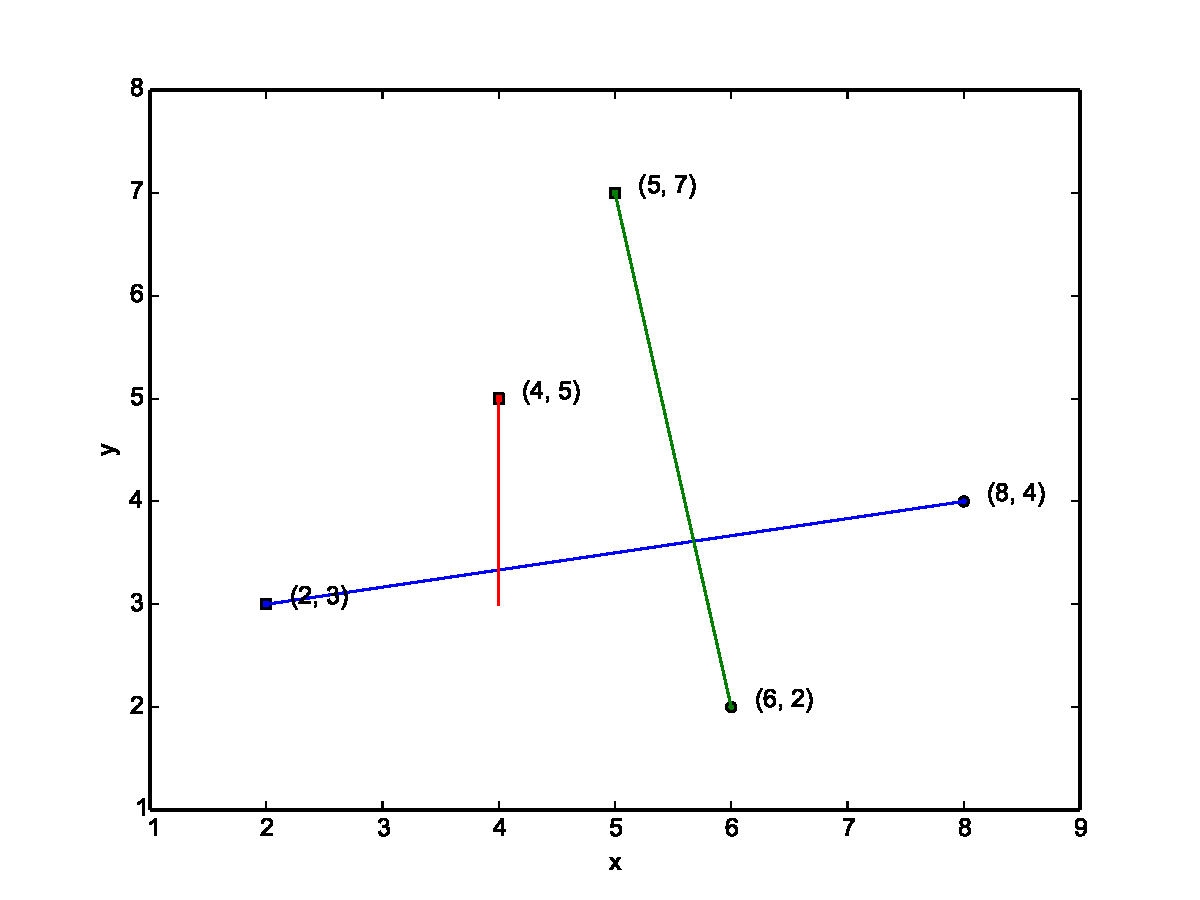
\includegraphics[width=0.85\textwidth]{img/ejemplos/ej3-4.pdf}
  \caption{\footnotesize Solución óptima para un conjunto dado de 5 puntos, donde no hay 3 puntos alineados.}
  \label{fig:ej3-4}
  \end{minipage}%
\end{figure}

Debido a que entre dos puntos siempre se puede establecer un semirrecta que los una, ningún conjunto de la partición solución, $P$, puede tener menos de dos elementos, salvo quizás uno (como ocurre en la figura (\ref{fig:ej3-3})). Si tuviera al menos dos conjuntos en $P$ con un solo elemento, $X$ y $X'$, entonces podría considerar $P'$, igual a $P$ salvo que tiene a $X'' = X \cup X'$ (que es válido porque seguro hay una semirrecta que una los dos puntos) y por lo tanto no posee a $X$ y $X'$. Claramente el cardinal de $P'$ es estrictamente menor al de $P$, lo que es un absurdo pues $P$ era solución. Luego, $P$ puede tener a lo sumo un conjunto con un elemento.

Por lo dicho en el párrafo anterior, se puede establecer una cota superior al cardinal de la solución cuando tengo $n$ puntos: $\lceil\frac{n}{2}\rceil$ ¿Cuándo se alcanza dicha cota? Cuando no existe ninguna semirrecta que pueda atravesar más de dos puntos. Una forma fácil de generar este tipo de casos es considerar $n$ puntos esparcidos sobre una circunferencia (una recta solo puede ser tangente o secante respecto a una circunferencia). En la figura (\ref{fig:ej3-5}) puede verse un ejemplo de esta situación para 16 puntos.

\begin{figure}[H]
  \centering
  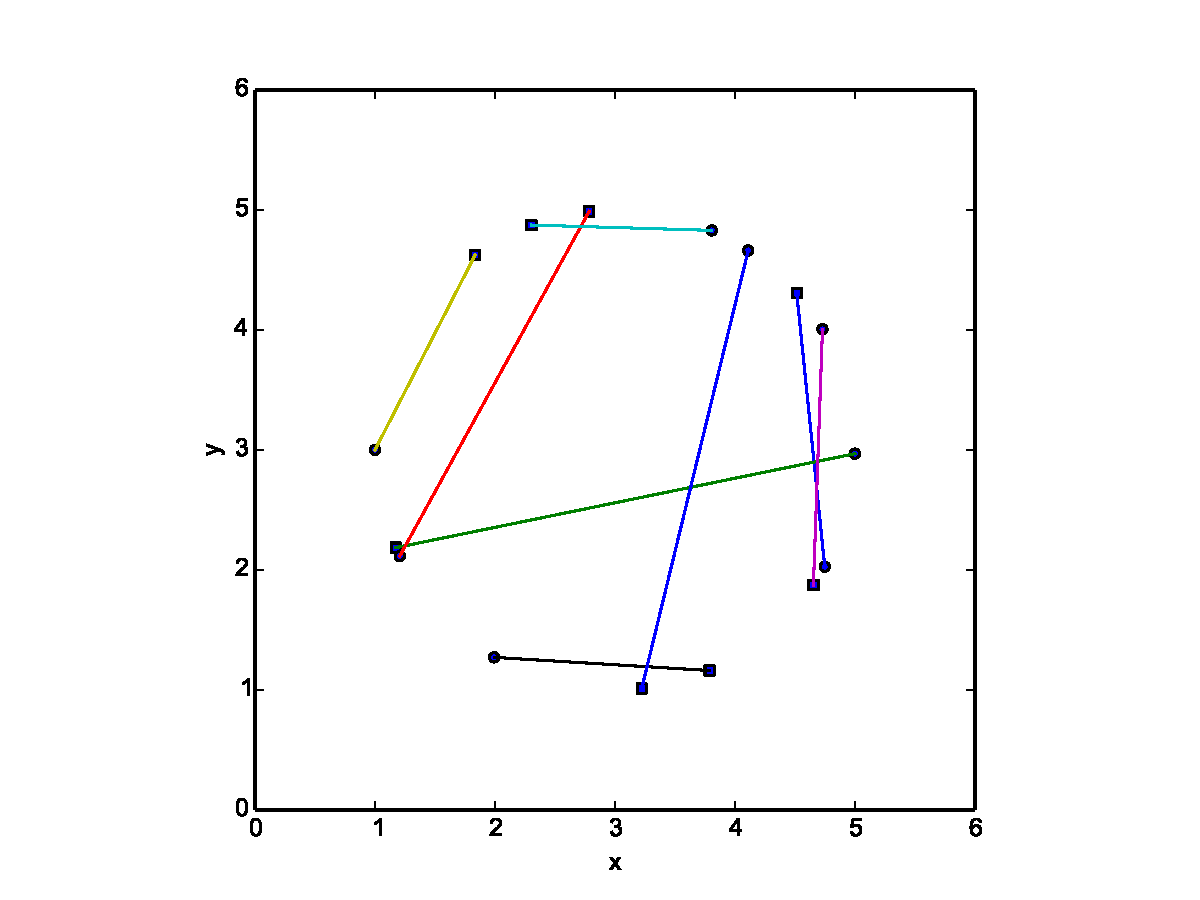
\includegraphics[width=0.65\textwidth]{img/ejemplos/ej3-5.pdf}
  \caption{\footnotesize Solución óptima para un conjunto de 16 puntos dispuestos sobre una circunferencia de radio 2 centrada en $(3,3)$.}
  \label{fig:ej3-5}
\end{figure}

\subsection{Explicación de la solución}
En esta sección daremos una explicación de por que el método de \texttt{backtracking} resulta correcto para resolver el problema presentado,  luego contaremos las podas y estrategias utilizadas, y finalmente presentaremos una explicación de las partes fundamentales de la implementación. 

En lo que sigue utilizaremos la siguiente terminología:
\begin{itemize}
  \item Solución: Es una partición $P$ de $C$ que satisface ambas condiciones del enunciado.
  \item Candidato a solución: Son las particiones de $C$ que satisfacen la segunda propiedad, aunque no necesariamente son de cardinal mínimo.
  \item Candidato a solución parcial: Es algún subconjunto de algún ``candidato a solución''. Es decir, es un conjunto de subconjuntos de $C$ tal que estos son disjuntos dos a dos, pero donde la unión de los mismos no es $C$. Siempre es posible extenderlo a un candidato a solución.
  \item Sucesor: Dado un ``candidato a solución parcial'', $X$, un sucesor del mismo es otro conjunto, $X'$, tal que $X'$ es o bien ``candidato a solución'', o bien ``candidato a solución parcial'', que cumple $X \subset X'$ (notar que la inclusión debe ser estricta).
\end{itemize}

\subsubsection{Árbol de posibilidades}
Los algoritmos de \textit{backtracking} son un refinamiento de los algoritmos de fuerza bruta por lo que pensemos primero la solución usando este método. Este último tipo de algoritmos consisten en enumerar todos los posibles candidatos a solución del problema y ver si satisfacen las condiciones pedidas o no. En nuestro caso particular, deberemos ver cuáles tienen cardinalidad mínima.

El proceso de construir las particiones se puede pensar como un árbol en el que en cada nivel se agrega un nuevo conjunto de los posibles a la partición que estoy armando. Así, en el nivel 0 (la raíz) tengo un conjunto vacío. En el nivel 1 tengo todos los subconjuntos de $C$ que verifican que existe alguna semirrecta que los une. Al escoger alguno de estos conjuntos lo agregamos en el candidato a solución parcial (o sea, obtenemos un sucesor). Debido a esto, en el nivel 2 tenemos un subconjunto de las posibilidades del nivel 1 estrictamente más pequeño pues debemos eliminar todas aquellas opciones que involucraban alguno de los puntos presentes en el conjunto previamente agregado (los conjuntos de la partición deben ser disjuntos). Se repite un procedimiento análogo hasta completar el candidato a solución, momento en el que estaremos parados en una hoja del árbol. 

Haciendo DFS (Depth-first search) recorremos todo el árbol de posibilidades, de forma que finalmente encontramos todas las particiones que cumplen la condición dos. Finalmente nos quedamos con alguna de cardinal mínimo (si hubiera más de una).

La correctitud de tal algoritmo es clara pues encuentra todo el universo de posibles soluciones, por lo que si efectivamente existe alguna eventualmente la obtiene. En particular, para todo conjunto finito es posible establecer particiones, así que siempre hay solución. 

La idea de \textit{backtracking} es preservar esta garantía de correctitud pero agilizando la búsqueda mediante la utilización de podas en el árbol de posibilidades. Dicho de otra forma, un algoritmo de este tipo descarta candidatos a soluciones parciales que a partir de algún criterio podemos predecir que no nos van a conducir a la solución. 

\subsubsection{Podas realizadas}
Una estrategia básica, basada en lo observado en la sección \ref{subsec:problema3}, es no considerar agregar conjuntos que tienen un solo elemento, salvo potencialmente en el último paso. Además, planteamos dos podas:

\begin{enumerate}
  \item Si actualmente estamos parados en un nodo de nivel $s$ (es decir que el cardinal de nuestro candidato a solución parcial es $s$) y anteriormente ya habíamos encontrado una solución en el nivel $s$, entonces no tiene sentido continuar por ese camino pues sabemos que todas los candidatos a soluciones a los que se arrive van a ser peores que un candidato previamente encontrado. De esta forma estamos ahorrándonos una búsqueda innecesaria y potencialmente muy costosa.
  \item Si actualmente estamos parados en un nodo de nivel $s$, y nos movemos a un sucesor en el nivel $s+1$ que resulta ser candidato a solución (y que debe ser mejor que el mejor que pudiéramos haber encontrado antes debido a la poda anterior), al volver al predecesor del nivel $s$ (DFS) no tiene sentido seguir probando con el resto de los sucesores pues no pueden dar candidatos a soluciones mejores que de tamaño $s+1$.
\end{enumerate}

La diferencia entre la poda 1 y 2 puede resultar un tanto sútil pero será más clara cuando veamos la implementación de \textit{backtracking}.

\subsubsection{Pseudocódigo}
  \paragraph{Variables globales:} Para tratar el problema definimos cuatro variables globales:
  \begin{itemize}
    \item \texttt{Vector(<int, int>)} $puntos$: almacena el conjunto de puntos. Dado que lo guardamos en un vector, se está imponiendo un orden sobre los puntos. Y como $puntos$ no se modifica nunca en el transcurso del programa (al menos después de inicializarlo), aprovecharemos dicho orden para referirnos a cada punto por el entero que representa su posición en $puntos$.
    \item \texttt{int} $n$: cantidad de puntos.
    \item \texttt{int} $mejor$: guarda el tamaño de la mejor partición hallada hasta el momento.
    \item \texttt{Vector(Vector(int))} $mejor\_sol$: guarda la mejor partición encontrada hasta el momento.
  \end{itemize}
  \paragraph{Clase Tablero:} La estructura \texttt{Tablero} nos permite condensar bien la información de la solución parcial que estamos desarrollando en un determinado momento junto con lo que necesitamos saber para hallar a sus sucesores. Las tres variables internas que tiene son:
  \begin{itemize}
    \item \texttt{Vector(Vector(int))} $solucion$: almacena una candidata a solución parcial hallada hasta el momento. Es decir que eventualmente $solucion$ es una partición de $puntos$, que puede ser efectivamente o no solución del problema planteado.
    \item \texttt{Vector(bool)} $vivos$: tiene tamaño $n$. $vivos[i] = true \Leftrightarrow$ el punto $i$ todavía no fue agregado en algún conjunto de $solucion$.
    \item \texttt{int} $cant\_vivos$: cantidad de puntos que todavía no fueron añadidos a $solucion$.
  \end{itemize}

  En cuanto a las funciones miembro de la clase, consideramos que el código es lo suficientemente simple y los nombres lo suficientemente descriptivos como para que sea necesaria una explicación detallada de cada uno.

  \paragraph{Función \texttt{solve}:} Es una función \textit{wrapper}, que se encarga esencialmente de llamar a la función $backtracking$, pasándole el tablero inicial correspondiente al nivel 0 del árbol de posibilidades (en el  que el candidato a solución parcial está vacío y tenemos todas las posibilidades disponibles). También se encarga de devolver la solución del problema.

  \begin{algorithm}[H]
  \begin{algorithmic}
  \caption{Pseudocódigo del procedimiento de \texttt{solve} en Kamehameha}
    \Procedure{solve}{\texttt{Vector(<int, int>)} $ptos$}$\rightarrow$ \texttt{Vector(Vector(int))}
      \State $Puntos\gets ptos$
      \Comment $O(n)$
      \State \texttt{Tablero} $inicial \gets Tablero()$
      \Comment $O(n)$
      \State $mejor \gets puntos.size()$
      \Comment $O(1)$
      \State $backtracking(inicial,0)$
      \Comment $O(T(n))$
      \State $return$ $mejor\_sol$
    \EndProcedure
  \end{algorithmic}
  \end{algorithm}

  \paragraph{Función de \texttt{backtracking}:} Es la función más importante de la solución. Toma como parámetros un Tablero $t$ y un entero $step$, que cumplen que el tamaño de $t.solucion$ es $step$.

  En las líneas 2 y 3 del pseudocódigo estamos realizando la primer poda: si el tamaño de $t.solucion$ (candidata a solución parcial) es mayor o igual que el de la mejor candidata a solución encontrada hasta el momento, entonces no continuamos analizando esta rama del árbol. Caso contrario, verificamos si ya tenemos completa la partición correspondiente. De serlo, por la poda anterior, estamos seguros de que es mejor que cualquier cosa que hubiéramos encontrado antes y por lo tanto actualizamos nuestras variables globales. 

  Si $t.solucion$ todavía no está completa, entonces queremos hallar todos los sucesores de $t$\footnote{Si bien definimos sucesor para hablar específicamente de las particiones resulta práctico usarlo en un sentido más amplio para hablar del tablero entero.}. Notar que tenemos dos sucesores por cada par de puntos disponibles (como se trata con semirrectas el orden si importa), pues únicamente consideramos semirrectas que pasen por al menos  dos puntos. Si solo quedase un punto entonces simplemente agregamos el conjunto que lo contiene a la solución parcial y obtenemos un candidato a solución. 

  Para recorrer todas estas posibilidades hacemos lo siguiente por cada punto disponible $i$: si es el único, agregamos el conjunto que solo lo contiene a él, y llamamos a $backtracking$ con el tablero actualizado y $step+1$; luego, retornamos. Si no era el único, entonces existe al menos un punto más con el que seguro se puede trazar una semirrecta. Por cada uno de estos puntos $j$, buscamos que otros puntos disponibles pertenecen a la semirrecta definida por $i$ y $j$ con origen en $i$. A todos estos puntos (incluidos $i$ y $j$) los metemos en un conjunto, y generamos un sucesor de $t$ que resulta de a una copia del mismo agregarle este conjunto nuevo\footnote{Notar que es fundamental que sea una copia de $t$, pues del mismo queremos obtener todos los posibles sucesores y por lo tanto no podemos modificarlo directamente.}. Finalmente, llamamos recursivamente a $backtracking$ con el sucesor y $step+1$.

  El procedimiento que realizamos para determinar si un punto $k$ pertenece a la semirrecta con origen en $i$ que pasa por $j$ es, por un lado ver si pertenece a la recta que pasa por $i$ y $j$, y luego ver si $k$ y $j$ están en el mismo cuadrante respecto de $i$ (un poco más adelante profundizamos esto útlimo). Notar que si $i$ y $j$ están alineados vertical (mismo $x$) u horizontalmente (mismo $y$), no se puede aplicar la fórmula clásica para determinar si un tercer punto pertenece a una recta dada por dos: $\frac{x_k-x_i}{x_j-x_i} = \frac{y_k-y_i}{y_j-y_i}$. Por lo tanto esos dos casos los analizamos a parte (el código usado para eso es muy simple de entender).

  Notemos que las líneas 25 y 26 aportan la segunda poda mencionada en la subsección anterior. La idea es que si al volver del llamado recursivo $mejor = s+1$, entonces no tiene sentido continuar ejecutando los ciclos pues todos los sucesores de $t$ van a ser de tamaño $s+1$ y por lo tanto no pueden mejorar lo que ya encontré. Podría parecer que esto se pisa con la condición de la línea 2 pero en rigor lo que nos ahorramos con la 25 es el costo de construir sucesores destinados a fracasar, cosa que no lográbamos de otra manera. Esto es particularmente útil en el mejor caso del algoritmo como veremos luego.
  
  \begin{algorithm}[H]
  \begin{algorithmic}[1]
  \label{algo:backtracking}
  \caption{Pseudocódigo del procedimiento de \texttt{backtracking} en Kamehameha}
    \Procedure{backtracking}{\texttt{Tablero} $t$, \texttt{int} $step$}
    \If {$step \geq mejor$}
    \Comment $O(1)$
      \State $return$
    \EndIf
    \If {$t.Solucionado()$}
    \Comment $O(n)$
      \State $mejor \gets step$
      \Comment $O(1)$
      \State $mejor\_sol \gets t.Solucion()$
      \Comment $O(n)$
    \Else
      \For {$i \in [0,..., n),$ $t.EstaVivo?(i)$}
      \Comment $n$ veces
        \If {$t.SoloQuedaUno?()$}
        \Comment $O(1)$
          \State $t.Matar(i)$
          \Comment $O(n)$
          \State $backtracking(t, step+1)$
          \State $return$
        \EndIf
        \For {$j \in [0,..., n),$ $j \neq i \land t.EstaVivo?(j)$}
          \Comment $n$ veces
          \State \texttt{Tablero} $sucesor \gets Copiar(t)$
          \Comment $O(2n+1)$
          \State \texttt{Vector(int)} $derrotados \gets [i, j]$
          \Comment $O(1)$ 
          \For {$k \in [0,..., n),$ $k \neq i \land k \neq j \land t.EstaVivo?(k)$}
          \Comment $n$ veces
            \If {$x_i \neq x_j \land y_i \neq y_j$}
            \Comment $O(1)$
              \If {$\frac{x_k-x_i}{x_j-x_i} = \frac{y_k-y_i}{y_j-y_i} \land MismoCuadrante?(i,j,k)$}
              \Comment $O(1)$
                \State $derrotados.push\_back(k)$ 
                \Comment $O(1)$ \footnotemark
              \EndIf
            \Else 
              \If {\footnotesize $(AlinHor?(i,j,k) \lor AlinVer?(i,j,k)) \land MismoCuadrante?(i,j,k)$}
              \Comment {\footnotesize $O(1)$}\normalsize
                \State $derrotados.push_back(k)$
                \Comment $O(1)$
              \EndIf
            \EndIf
          \EndFor
          \State $sucesor.Matar(derrotados)$
          \Comment $O(n)$
          \State $backtracking(sucesor, step+1)$
          \If {$mejor = s+1$}
            \Comment $O(1)$
            \State $return$
          \EndIf
        \EndFor
      \EndFor
    \EndIf
    \EndProcedure
  \end{algorithmic}
  \end{algorithm}

  \footnotetext{En general, hacer push\_back a un vector tiene peor caso $n$. Sin embargo en el código usamos la función reserve (\url{http://www.cplusplus.com/reference/vector/vector/reserve/}) que permite que la operación sea constante siempre que no agreguemos más de $n$ elementos, cosa que obviamente no puede ocurrir.}

  \paragraph{Función \texttt{mismoCuadrante}:} Su código en si no es particularmente interesante, lo importante es entender la idea. El punto $i$ es el origen de la semirrecta que estamos analizando. En particular, podemos pensar que este punto genera cuatro cuadrantes respecto de él (del mismo modo que lo hace el origen de coordenadas). Por lo tanto, lo que hace esta función es chequear si los puntos $j$ y $k$ están en el mismo cuadrante respecto de $i$. Si no lo estuvieran, entonces por más que estén alineados no pueden pertenecer a la misma semirrecta con origen en $i$.

\subsection{Complejidad del algoritmo}
\subsubsection{Complejidad en peor caso}
El peor caso como vimos es cuando no hay tres o más puntos alineados. En tal situación la partición solo estará compuesta por conjuntos de dos puntos (y uno de un elemento si $n$ es impar), por lo que tendrá cardinalidad igual a $\frac{n}{2}$. Por lo tanto, todas las hojas de nuestro árbol estarán a distancia $\frac{n}{2}$ de la raíz. Entonces nuestro algoritmo recorrerá todas las ramas hasta el fondo. Bueno, en rigor esto no es exactamente así debido a las podas. No obstante omitiremos ese detalle en el cálculo de la complejidad, y asumiremos la primer situación pues es al menos tan mala y por lo tanto permite acotar la complejidad de nuestro algoritmo.

La complejidad total del algoritmo es la complejidad de \texttt{solve}, $O(n + T(n)) = O(max\{n, T(n)\})$. Veamos entonces cuál es la cota superior de complejidad en peor caso de \texttt{backtracking}. 

\paragraph{Ecuación de recurrencia}
Primero debemos dar la ecuación de recurrencia, $T$, para la cantidad de operaciones que realiza $backtracking$ con un input de tamaño $n$ en el peor caso. Tal ecuación, basados en las complejidades anotadas en el algoritmo \ref{algo:backtracking}, es la siguiente

\begin{equation}
 \label{eq:aqui-le-mostramos-como-hacerle-la-llave-grande}
 T(n) = \left\{
     \begin{array}{ll}
 1      & \mathrm{si\ } n = 0 \\
 9      & \mathrm{si\ } n = 1 \\
 n^3 + n^2\times T(n-2) & \mathrm{si\ } n \geq 2
     \end{array}
   \right.
\end{equation}

Decidimos omitir las constantes que suman y multiplican en el caso $n\geq 2$ pues solo harán más engorrosas las cuentas en la demostración y no modifican la complejidad.

A continuación damos una fórmula cerrada para esta ecuación de recurrecia cuando $n$ es par\footnote{Para $n$ impar puede obtenerse una fórmula muy parecida, reemplazando el $T(0)$ por $T(1)$ y cambiando $\frac{n}{2}$ por $\frac{n-1}{2}$. Para evitar sobrecargar la demostración nos limitamos al caso par pero el impar es análogo.}:

\paragraph{Lema 3.1:} 
\begin{equation}
\begin{aligned}
  F(n) &= \sum_{i=0}^{\frac{n}{2}-1} \left((n-2i) \prod_{j=0}^{i}(n-2j)^2\right) + \left(\prod_{i=0}^{\frac{n}{2}-1}(n-2i)^2\right) T(0)\\
  &= \sum_{i=0}^{\frac{n}{2}-1} \left((n-2i) \prod_{j=0}^{i}(n-2j)^2\right) + \prod_{i=0}^{\frac{n}{2}-1}(n-2i)^2
\end{aligned}
\end{equation}

Una demostración de este lema puede encontrarse en el apéndice.

  Ahora acotemos $F(n)$, con $n \geq 2$:
  \begin{equation}
  \begin{aligned}
  F(n) &= \sum_{i=0}^{\frac{n}{2}-1} \left((n-2i) \prod_{j=0}^{i}(n-2j)^2\right) + \prod_{i=0}^{\frac{n}{2}-1}(n-2i)^2 \\
  &\leq \sum_{i=0}^{\frac{n}{2}-1} \left(n \prod_{j=0}^{i}n^2\right) + \prod_{i=0}^{\frac{n}{2}-1}n^2 \\
  &= \sum_{i=0}^{\frac{n}{2}-1} (n^{2i+1}) + n^{2\times(\frac{n}{2}-1)} \\
  &= \sum_{i=0}^{\frac{n}{2}-2} (n^{2i+1}) + n^{n-1} + n^{n-2} \\
  &\leq \sum_{i=0}^{\frac{n}{2}-2} (n^{n-1}) + n^{n-1} + n^{n-1} \\
  &\leq \frac{n}{2} n^{n-1} 
  = \frac{1}{2} n^{n}
  \end{aligned}
  \end{equation}

  Como $n \geq 2$, esto último está bien definido (solo se invalida en 0).

  Luego, por definición de $O$, $F(n) = T(n)$ es $O(n^n)$. Como $n^n\leq n^{n+2} (\forall n \in \mathbb{N})$, entonces $O(n^n)\subset O(n^{n+2})$, y $T\in O(n^{n+2})$. Dado que la complejidad total del algoritmo era $O(max\{n, T(n)\})$, entonces la misma resulta $O(n^{n+2})$, que era la complejidad pedida.

\subsubsection{Complejidad en mejor caso}

El mejor caso es indudablemente el caso en que todos los puntos están alineados y el primer punto del vector $puntos$ es uno de los puntos extremos, es decir que basta con una semirrecta con origen en ese punto para atravesar todos. En tal situación, solo se entrará una vez a los ciclos de las líneas 8 y 13 (esto es debido a la segunda poda), y $n$ al de la 16.

Si hacemos el seguimiento línea por línea en el pseudocódigo, vemos que la complejidad total será $O(1+n+2+1+(2n+1)+1+3\times n+n+1+n) = O(n)$, por álgebra de órdenes.

Notar que si la línea 25 no estuviera, pese a haber encontrado obviamente la mejor solución posible, se seguiría iterando sobre todos los sucesores, con lo que la complejidad terminaría siendo $O(n^3)$. 

\subsection{Performance del algoritmo}

Como vimos anteriormente, el algoritmo tiene una complejidad de $O(n^{n+2})$. Sin embargo, esta cota no era ajustada. Veamos si esto se refleja en la realidad. El primer caso que analizaremos es el peor caso, es decir, aquel en el que siempre se necesitan $\frac{n}{2}$ rectas, el máximo posible.

\begin{figure}[H]
 \centering
	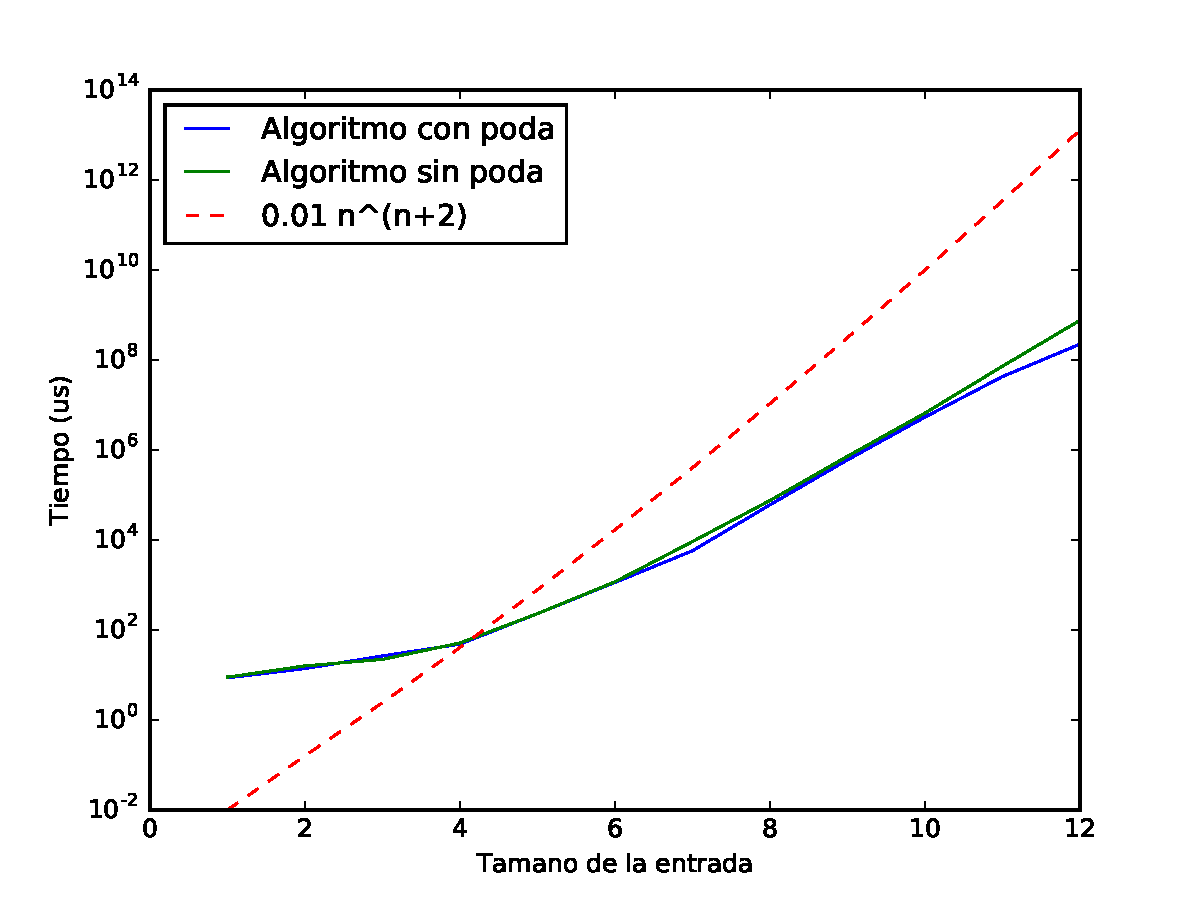
\includegraphics[width=0.8\textwidth]{img/tiempos/kamehameha1.pdf}
	\caption{\footnotesize Tiempo que toma el algoritmo en $\mu$s para una entrada de tamaño $n$.}
	\label{fig:kamehameha-tiempos1}
\end{figure}

Como puede verse, el tiempo requerido por el algoritmo crece muy aceleradamente, razón por la cual debimos analizarlo hasta $n = 12$; en tal situación, cada corrida tardaba alrededor de 15 minutos (Nótese que si $n = 12$, entonces $n^{n+2} \equiv 10^{15}$).

Como este es el peor caso, la poda no contribuye en nada, dado que hay que recorrer cada posibilidad de entre todas las combinaciones. Esto se refleja claramente en el gráfico.

Analicemos ahora el caso promedio.

\begin{figure}[H]
 \centering
	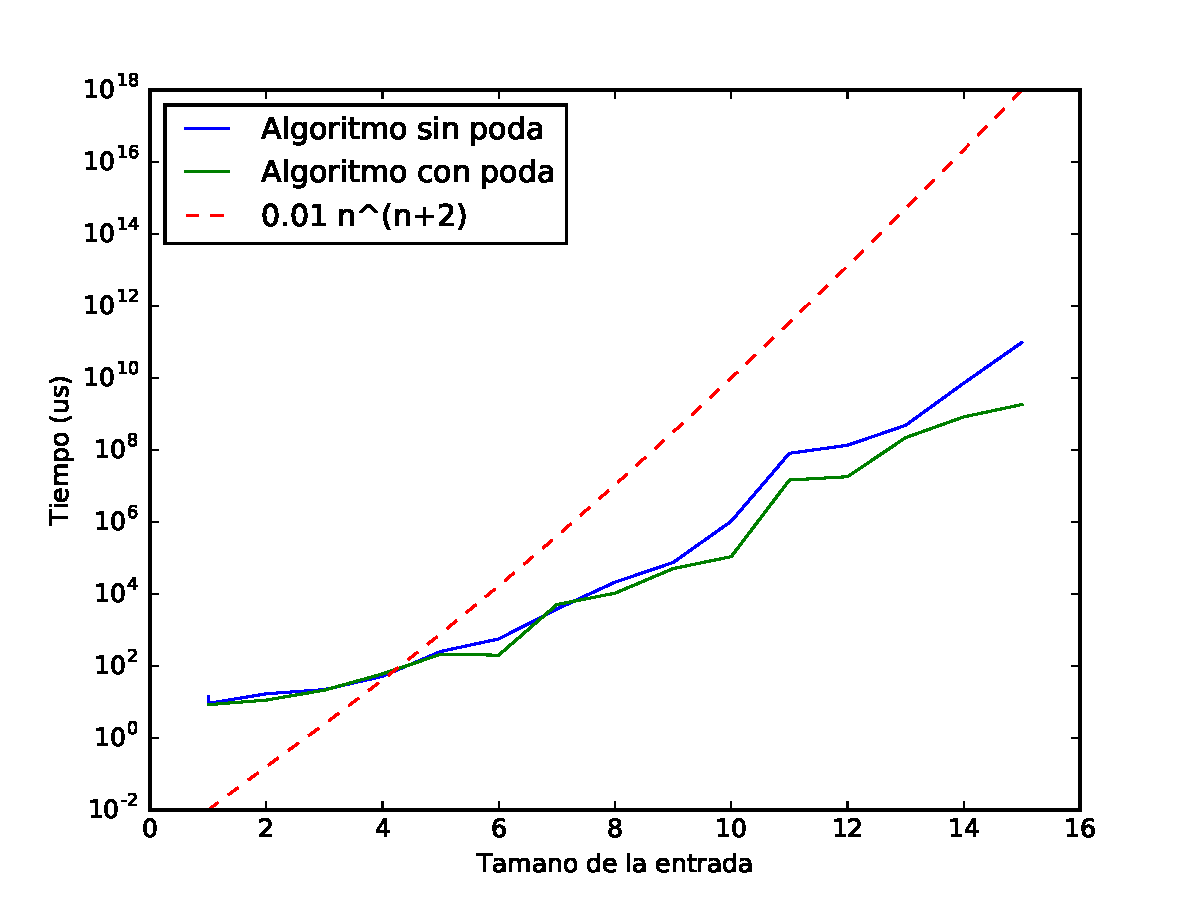
\includegraphics[width=0.8\textwidth]{img/tiempos/kamehameha2.pdf}
	\caption{\footnotesize Tiempo que toma el algoritmo en $\mu$s para una entrada de tamaño $n$.}
	\label{fig:kamehameha-tiempos2}
\end{figure}

Como puede verse en la figura \ref{fig:kamehameha-tiempos2}, el caso promedio es muy similar al peor caso. Esto se debe, a que lo más probable es que se necesiten $\frac{n}{2}$ rectas para cubrir a todos los puntos. Esto se prueba en el ap\'endice.

Por último, analicemos el mejor caso. El mejor caso es, obviamente, en el que se necesita una sola recta para cubrir a todos los puntos, y esta recta se encuentra en el primer intento. Como vimos antes, en este caso la complejidad del algoritmo es de $O(n)$. Veamos si esto se confirma experimentalmente.

\begin{figure}[H]
 \centering
	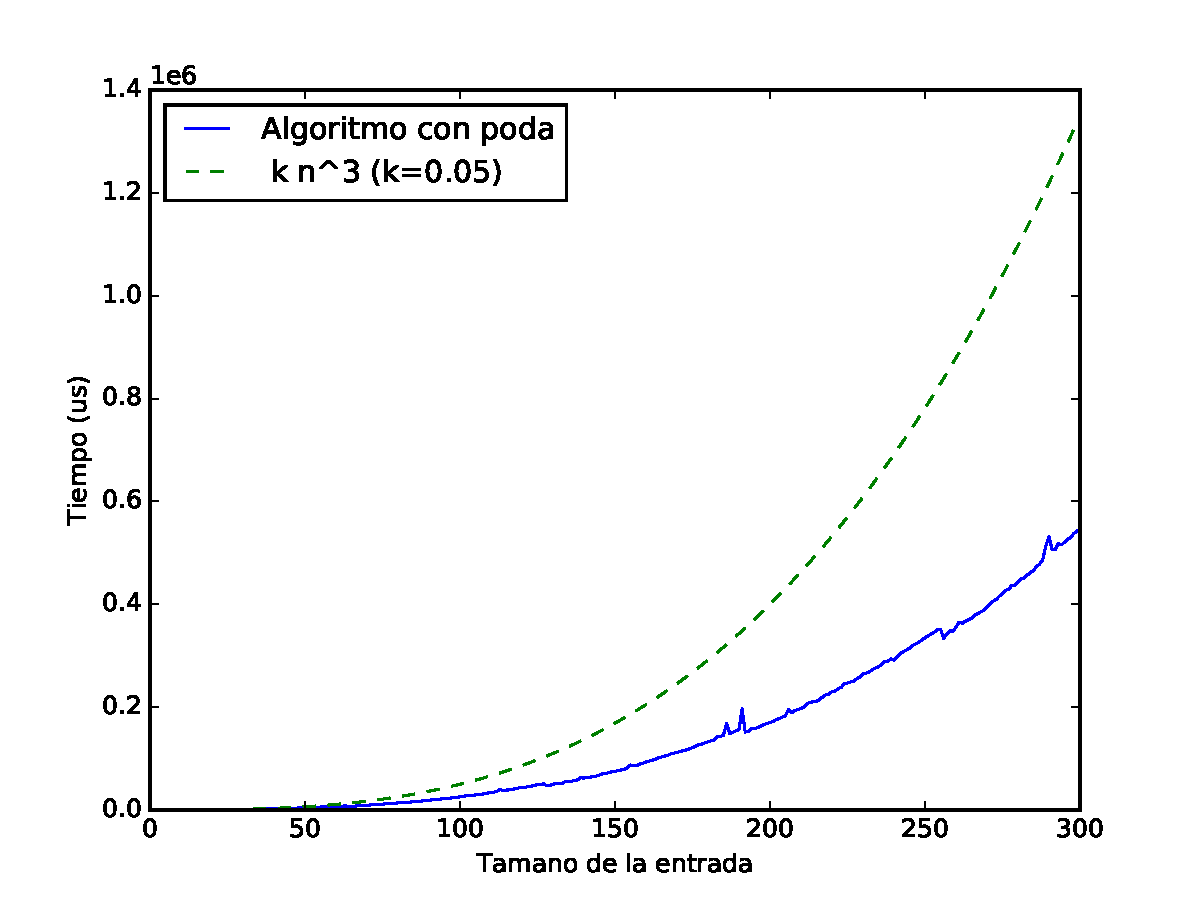
\includegraphics[width=0.8\textwidth]{img/tiempos/kamehameha3.pdf}
	\caption{\footnotesize Tiempo que toma el algoritmo en $\mu$s para una entrada de tamaño $n$.}
	\label{fig:kamehameha-tiempos3}
\end{figure}

\begin{figure}[H]
 \centering
	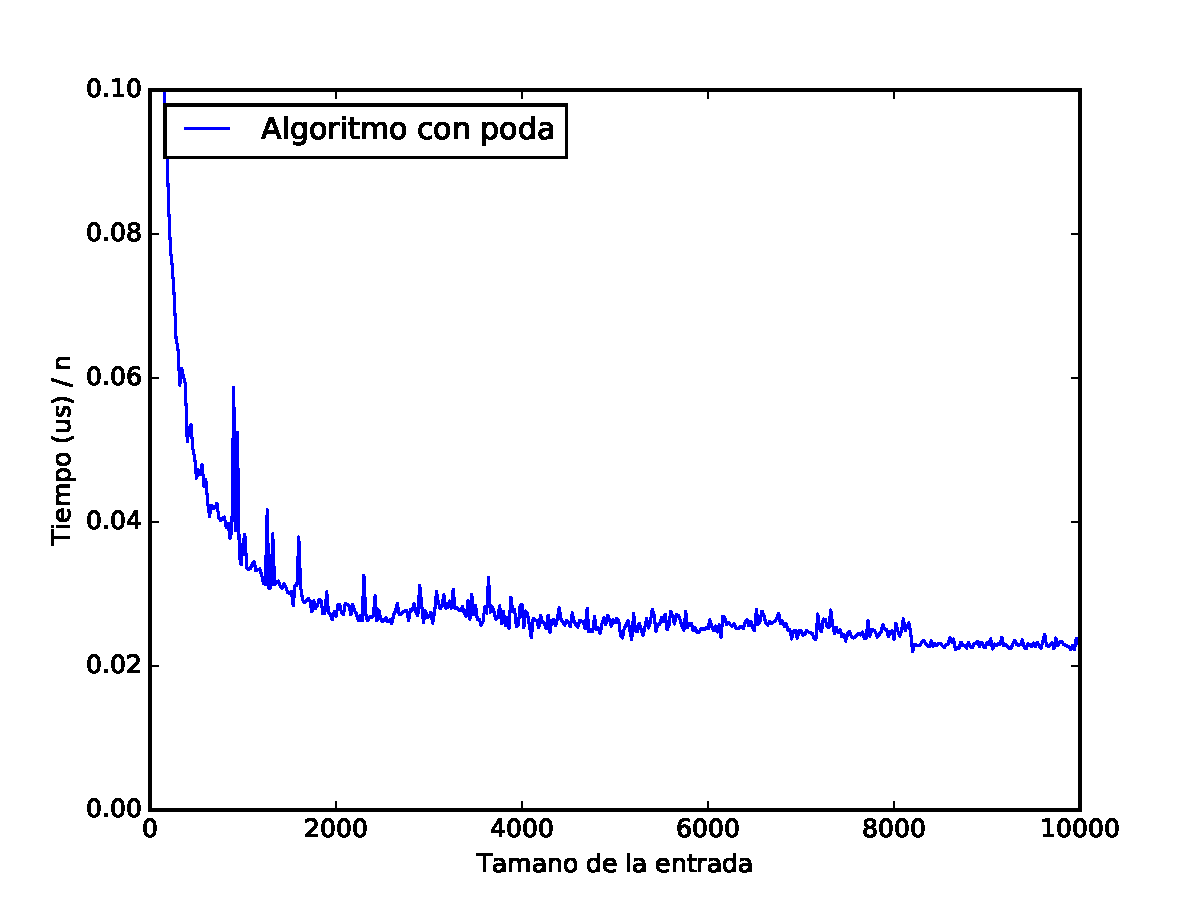
\includegraphics[width=0.8\textwidth]{img/tiempos/kamehameha4.pdf}
	\caption{\footnotesize Tiempo que toma el algoritmo en $\mu$s para una entrada de tamaño $n$.}
	\label{fig:kamehameha-tiempos4}
\end{figure}

Efectivamente, se ve que la complejidad del algoritmo es de $O(n)$. La disminución del tiempo de ejecución alrededor de $n = 8200$ no pudo ser explicada por nosotros. Dado que 8192 es una potencia de 2, podemos inferir que tiene que ver con un tema de \emph{cache} al almacenar los datos en memoria.

\subsubsection{M\'etodo de experimentación}

Para el peor caso, para asegurarnos que siempre se requirieran exactamente $\frac{n}{2}$ rectas para cubrir todos los puntos, tomamos $n$ puntos sobre una circunferencia (específicamente, sobre la circunferencia de radio $\frac{n}{2}$ con centro en el $(n,n)$). Nótese que (por la definición de circunferencia) no hay 3 puntos en la misma recta, por lo tanto necesitaremos $\frac{n}{2}$ rectas para cubrir todos los puntos.

El caso promedio se genera de manera similar al problema anterior. Para cada $n$, elegimos $n$ puntos al azar de la grilla $\{1,..., n^2\} \times \{1, ... , n^2\}$.

Estos puntos eran elegidos al azar usando el mismo \emph{seed} cada vez (para la instancia 1 usábamos 1 como seed, para la instancia 2, usábamos 2, etc.), de tal manera que los experimentos fueran reproducibles de una manera válida.
La cantidad de instancias que creamos para cada $n$ fue 40.
Cada instancia fue ejecutada 20 veces, y el resultado final era el mínimo de todas las corridas.
Luego, tomábamos la mediana de todas las instancias. Es decir, el restultado final es la mediana de los mínimos.

Finalmente, para el mejor caso, el caso de tamaño $n$ estará formado por los puntos $\{(1,1), (2,2), \cdots, (n, n)\}$, en ese orden, de tal manera que el backtracking tome a los puntos $(1,1)$ y $(2,2)$ en su primer intento, y ese intento sea el exitoso.
